\subsection{Three independent sources and one
protocol}\label{three-independent-sources-and-one-protocol}

The empirical study uses three independently collected EEG sources. They
span a wide spread of acquisition and protocol differences, so the
recovered label is interpreted only as a source-associated technical
mixture, and no claim is made that a single device or task can be
isolated as the cause.

The first source is a research-grade BrainVision study with eight
channels at a thousand hertz, thirty-two subjects and sixty-four
recordings. The second is a consumer-grade Emotiv headset with fourteen
channels at a hundred and twenty-eight hertz, thirty subjects and thirty
long recordings. The third is the eyes-open baseline run R01 of the
PhysioNet \emph{EEG Motor Movement/Imagery Dataset} (eegmmidb), a
hundred and nine subjects and sixty-four channels.

All three are reduced to one pre-specified pipeline before any
clustering. Four shared channels are retained, F3, F4, O1, and O2; the
data are resampled to a hundred and twenty-eight hertz, common-average
referenced, band-passed from one to forty hertz with a fifty-hertz
notch, and cut into four-second windows. Window covariances use
Ledoit--Wolf shrinkage and are linearized through the matrix logarithm,
and the recording feature is the unweighted within-recording average.
The protocol is fixed before analysis, and each recording receives one
equal vote. The source-level facts are stated in
Table~\ref{tab:sources}; the complete data processing,
versions, links, and call parameters are in Supplementary S1.

\begin{table}[htbp]
\centering
\small
\caption{The three independently collected EEG sources and their acquisition characteristics. The harmonized pipeline reduces these heterogeneous sources to a common feature space.}
\label{tab:sources}
\begin{tabular}{lllll}
\hline
source (accession) & device & channels & rate & subjects/recordings\\
\hline
ds007541 & BrainVision & 8 & 1000 Hz & 32 / 64\\
ds008099 & Emotiv EPOC & 14 & 128 Hz & 30 / 30\\
on004362 & PhysioNet R01 & 64 & 160 Hz & 109 / 109\\
\hline
\end{tabular}

\end{table}

The recording is the unit of feature construction and of the primary
clustering. Windows estimate a recording's feature and never carry their
own p-values. A separate analysis treats the subject as the independent
unit. All permutation tests use a one-sided upper tail with the plus-one
correction, \(p=(1+\#\{b:T_b\ge T_{\rm obs}\})/(B+1)\), and the smallest
reportable value is \(1/(B+1)\). Each p-value is labeled with its
resampling count and its unit.

The analyses separate into a primary set and a secondary exploratory
set. The primary set is the balanced oracle-\(K\) recovery, the blind
\(K\) selection, the unbalanced full-pool fit, and the subject-level
aggregation, all on the covariance features with the recording as the
unit unless stated. The secondary set in Section 7.5 covers alternative
spatial representations, channel-drop checks, novelty detection,
non-covariance phase locking, and component ablations. No prespecified
multiple-comparison strategy is applied across these analyses, and the
permutation \(p\)-values, ARI figures, and bootstrap intervals are
descriptive diagnostics, not confirmatory hypothesis tests with a
family-wise error guarantee.

Before the clustering results, one caveat frames what a recovered label
can mean. The source labels are fully predictable from recording
metadata alone, the window count ranges having no overlap across the
three sources, so the partition the method recovers is a technical
source-associated structure, not a latent biological environment. The
detailed controls and the feature-to-metadata correlations are in
Section 7.2.

\subsection{Metadata controls}\label{metadata-controls}

A direct diagnostic asks whether the sources are already separated by
information unrelated to latent environments. The number of windows is
nine for every recording in the first source, fifteen in the third, and
ranges from eighty to a hundred and fourteen in the second; the three
ranges do not overlap. A decision tree given only this field predicts
the source with perfect cross-validated accuracy. Subject-grouped folds,
which keep every recording of one subject in a single fold across the
171 subject groups, also give accuracy one, so the result is not
produced by related recordings crossing between folds. Adding the device
metadata constant within a source holds the accuracy at one for both
logistic and tree models. The sources are therefore fully separable from
trivial metadata alone, the clearest evidence that the recovered label
is a technical one.

The association with metadata is quantified rather than asserted. Across
the ten covariance features, the absolute correlation with window count
reaches \(0.663\) and averages \(0.210\). A length-matched control would
be natural, but the data do not permit one. The three window-count
ranges have no common support, and trimming to an overlap would leave an
empty design. We state this as an infeasibility rather than replace it
with a different control.

Two controls check where the structure appears. The same-device control
pools recordings within one source and repeats the clustering there. The
silhouette stays low, between \(0.18\) and \(0.22\), and the clustering
agrees with the subject label at an ARI of only \(0.02\) to \(0.03\), so
no stable within-device structure is recovered. The same-task control
keeps the two resting sources and drops the third; despite the shared
task they still separate at two clusters, with a balanced ARI of
\(0.53\), \(0.56\) over three seeds. A shared task category is therefore
not sufficient to remove the source difference, but the controls cannot
name a single driver because device, population, length, reference, and
preprocessing still differ together. The full metadata table is in
Supplementary S3.

\subsection{Recovery under a known number and blind
selection}\label{recovery-under-a-known-number-and-blind-selection}

\begin{figure}[htbp]
\centering
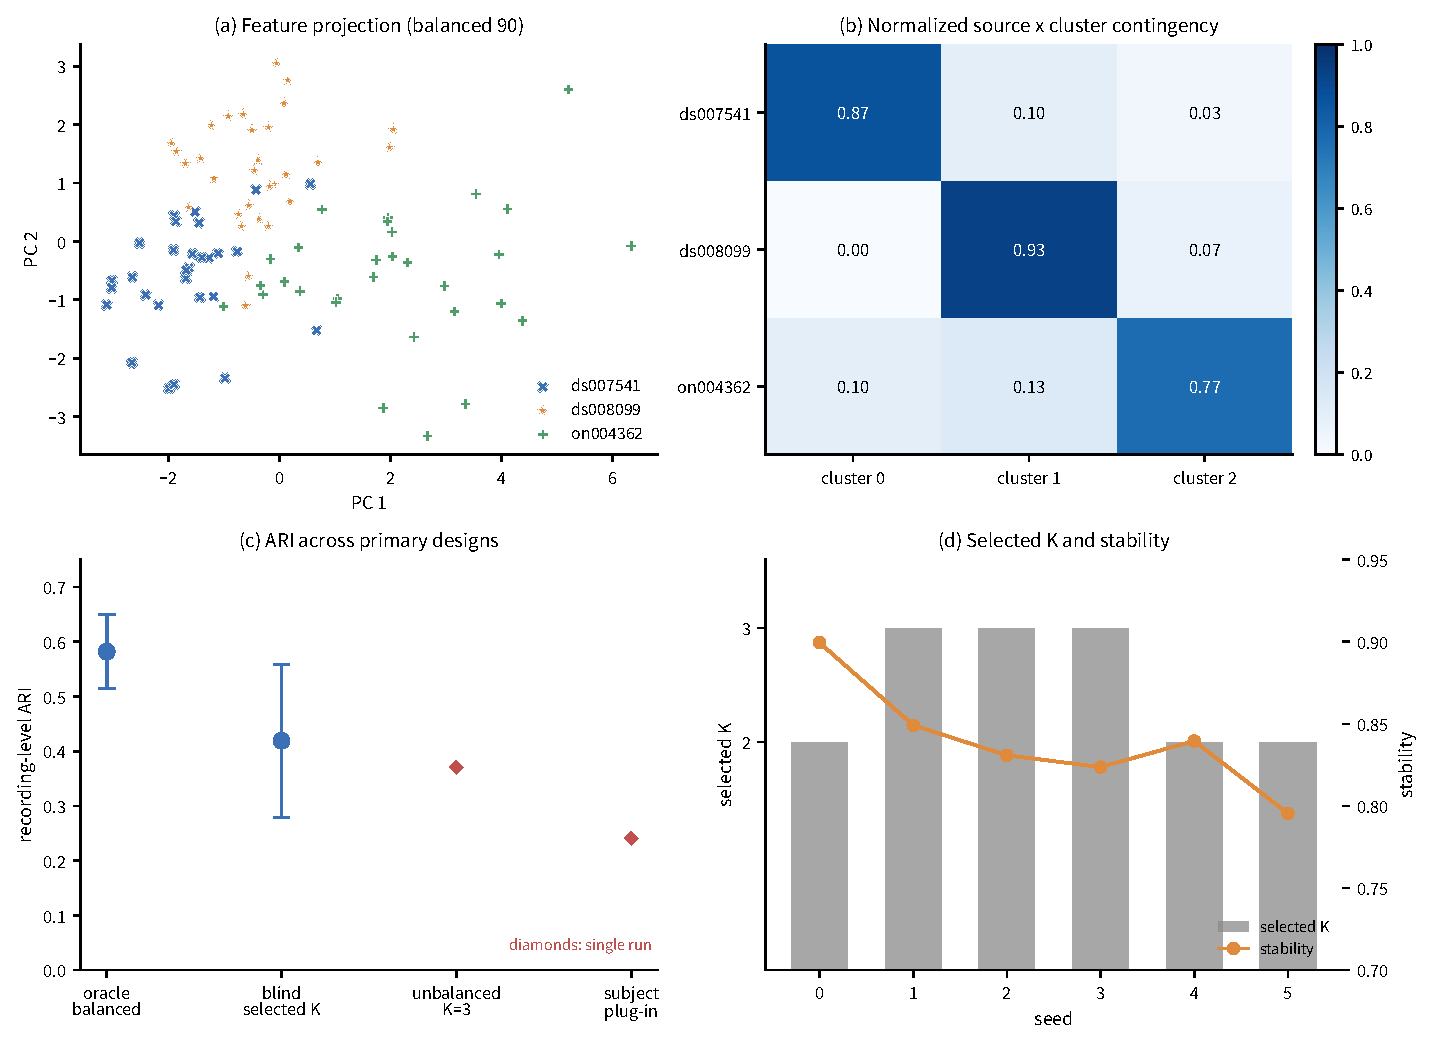
\includegraphics[width=\textwidth]{fig8_main_results.pdf}
\caption{Four-panel main EEG result. (a) Two-dimensional PCA projection of the balanced ninety-recording features, colored by source. (b) Source x cluster contingency at the oracle value $K=3$, normalized within each source, with the diagonal dominant. (c) Recording-level ARI across the four primary designs, with mean and standard deviation for the multi-seed designs and diamonds for single-run realizations. (d) Blind selector: selected $K$ (bars) and bootstrap stability (line) across six balanced seeds. The figure consolidates evidence otherwise spread across the tables and the supplementary.}
\label{fig:main}
\end{figure}

The clearest positive evidence comes from the balanced cross-source
design. With only two sources pooled, every paired combination is
recovered, with ARI between \(0.48\) and \(0.64\). Pooling all three
sources at the oracle value of three strengthens the result. On the
balanced ninety-recording design, recording-level ARI reaches \(0.608\),
and the result holds across six balanced seeds at a mean of \(0.582\),
as detailed in Table~\ref{tab:perseed}.

\begin{table}[htbp]
\centering
\small
\caption{Per-seed recording-level ARI on the ninety-recording balanced design and on the cross-fitted held-out construction, with the sample mean and standard deviation reported rather than a mean alone. The cross-fitted column is defined in Supplementary S1.}
\label{tab:perseed}
\begin{tabular}{lcc}
\hline
seed & balanced $K=3$ ARI & cross-fitted $K=3$ ARI\\
\hline
0 & 0.608 & 0.602\\
1 & 0.589 & 0.630\\
2 & 0.476 & 0.602\\
3 & 0.535 & 0.717\\
4 & 0.607 & 0.617\\
5 & 0.675 & 0.493\\
\hline
mean & 0.582 & 0.610\\
std & 0.068 & 0.072\\
\hline
\end{tabular}

\end{table}

The balanced design is not a blind run. Thirty recordings are drawn from
each source, and the source label is used only to select the recordings;
it never enters the covariance features, the scaler, or the clustering.
The draw and the rule are fixed in advance, so this is a pre-specified
evaluation. It is recording-level, oracle-\(K\) evidence that the source
label can be reconstructed from the covariance features, not an external
validation of the blind pipeline and not a subject-level claim.

The prespecified blind selector does not reproduce the oracle result. On
the seed-0 balanced design it returns two clusters rather than three,
with ARI \(0.279\). Run across all six balanced seeds, the automatic
choice is not fixed: it selects \(K=2\) in three seeds and \(K=3\) in
the other three, and the ARI measured at the selected \(K\) averages
\(0.419\pm0.140\). What stays systematic is the two-cluster geometry.
Whenever \(K=2\) is fitted, the same two sources, ds007541 and ds008099,
are joined, while on004362 stays apart, and the merged cluster separates
cleanly into the two true components once the correct number is
restored. The forced two-cluster ARI averages \(0.277\pm0.043\) across
the seeds. The stability gate drives the under-selection, not the BIC
term, which on its own prefers the larger values, and no prespecified
rule recovers the oracle number on every seed. We present this as a
primary finding rather than a caveat. Covariance structure can be
recoverable at a fixed \(K\) while the number of sources is itself not
reliably selected by the blind procedure. The \(K\) sensitivity across
the full grid is shown in Figure~\ref{fig:ksens}, and
the per-seed numbers are in Table~\ref{tab:blind}.

\begin{table}[htbp]
\centering
\small
\caption{Per-seed blind selection on the balanced ninety-recording design. Each balanced seed uses a fresh \texttt{default\_rng(2026)} for the clustering randomness. The automatic choice is unstable, two clusters in three seeds and three in the other three, but forcing two clusters always merges the same pair, ds007541 and ds008099, with on004362 kept mostly apart. Stability is the bootstrap cluster-agreement at the selected $K$. Alternative RNG constructions retain the same pattern and never select $K=3$ in all six seeds.}
\label{tab:blind}
\begin{tabular}{ccccc}
\hline
seed & selected $K$ & ARI at selected $K$ & forced $K=2$ ARI & stability\\
\hline
0 & 2 & 0.279 & 0.279 & 0.899\\
1 & 3 & 0.589 & 0.326 & 0.849\\
2 & 3 & 0.476 & 0.225 & 0.831\\
3 & 3 & 0.561 & 0.225 & 0.824\\
4 & 2 & 0.296 & 0.296 & 0.840\\
5 & 2 & 0.313 & 0.313 & 0.795\\
\hline
\end{tabular}

\end{table}

\begin{figure}[htbp]
\centering
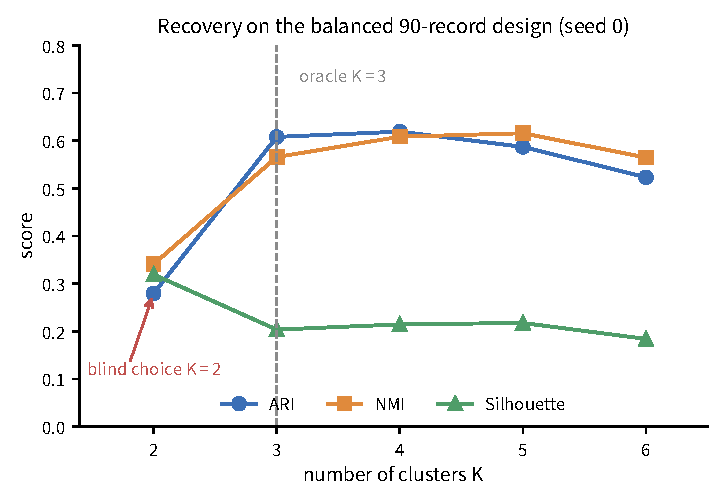
\includegraphics[width=0.85\columnwidth]{fig1_k_sensitivity.pdf}
\caption{This figure compares candidate-$K$ diagnostics with the prespecified oracle evaluation value $K=3$; it does not establish that $K=3$ is identifiable from the pooled data. The adjusted Rand index, normalized mutual information, and silhouette are reported across $K=2,\dots,6$ on the balanced ninety-recording design. The blind selector stops at two clusters with ARI $0.279$, the oracle value of three gives $0.608$, and the scores plateau before declining as extra clusters split the sources.}
\label{fig:ksens}
\end{figure}

\subsection{Balance and subject-level
uncertainty}\label{balance-and-subject-level-uncertainty}

The balanced design does real work, and removing it lowers the point
estimate. On the full unbalanced pool the recording-level ARI falls to
\(0.371\). The most direct plug-in, run once over all subjects without
resampling, is weaker still. With a hundred and seventy-one subjects in
unequal group sizes, the subject-level ARI is only \(0.241\). The large
source is split across several clusters and the small sources merge, the
same mechanism seen in the unbalanced recording result. Balance is
therefore a condition for recovery, not a cosmetic detail. The four
primary designs are consolidated in
Table~\ref{tab:designs}.

\begin{table}[htbp]
\centering
\small
\caption{ARI across the four primary designs, with the statistical scope stated for each row. The balanced oracle-$K$ design is the strongest; the blind selector is seed-dependent and does not recover the oracle number, while unbalanced pooling and the subject plug-in weaken further.}
\label{tab:designs}
\begin{tabular}{lllll}
\hline
design & $K$ & balance & unit & ARI\\
\hline
oracle-$K$ (DELVE-G) & 3 & balanced & recording & $0.582\pm0.068$\\
blind selector (DELVE-B) & 2 or 3 & balanced & recording & $0.419\pm0.140$\\
fixed $K=3$ & 3 & unbalanced & recording & $0.371$\\
full plug-in & selected & unbalanced & subject & $0.241$\\
\hline
\multicolumn{5}{@{}p{\textwidth}@{}}{\footnotesize Seed-averaged rows report mean$\pm$standard deviation across six prespecified balanced seeds.}\\
\multicolumn{5}{@{}p{\textwidth}@{}}{\footnotesize The oracle row reaches $0.608$ at seed 0. The blind selector chose $K=2$ in three seeds and $K=3$ in three, and the reported ARI is taken at the selected $K$; the per-seed detail is in Table~\ref{tab:blind}.}\\
\multicolumn{5}{@{}p{\textwidth}@{}}{\footnotesize The unbalanced and plug-in rows are single realizations, not seed averages.}\\
\end{tabular}

\end{table}

Treating the subject as the independent unit, a subject-cluster
bootstrap with five hundred resamples confirms the balanced recovery
does not rest on treating repeated recordings as independent. The
subject-aggregated bootstrap gives a mean of \(0.616\) with a
ninety-five percent interval from \(0.31\) to \(0.81\), the
cluster-preserving design gives \(0.554\) with a wider interval, and the
naive recording bootstrap gives \(0.603\). All three intervals exclude
zero. The single balanced subject realization at seed zero is \(0.523\),
a single draw from the same resampling mechanism rather than a point
estimate on its own. The intervals are percentile intervals, not BCa,
and they are finite-sample diagnostics without a coverage theorem. The
full resampling protocol and the bootstrap figure are in Supplementary
S4.

\subsection{Secondary analyses}\label{secondary-analyses}

Alternative spatial representations test whether the recovery is an
artifact of the reference or of one channel. A reference-free bipolar
montage lowers the balanced ARI to \(0.415\), and a surface Laplacian
raises it to \(0.678\), both clearly positive. Dropping any one of the
four shared channels leaves ARI between \(0.34\) and \(0.42\), so no
single channel drives the result, though distributed bad channels or a
shared device fingerprint are not excluded. Recovery persists across
representations while its magnitude is representation-dependent, and
strict reference invariance is not claimed.

Pooled label recovery does not establish generalization to unseen data.
Each source is held out in turn, the scaler and two centers are fitted
on the other two and frozen, and the held-out recordings are mapped
without a refit. Two held-out sources are clearly detectable as novel,
with ROC AUC between \(0.89\) and \(0.93\), while the third is weakly
separated at \(0.70\). When all three sources enter training, a
cross-fitted fold assigns held-out recordings with ARI \(0.610\),
matching the transductive \(0.608\) and corresponding to the
sample-split mechanism in the theory. Novelty detection is not the same
as correctly labeling a new environment, and full cross-domain
generalization remains unproved.

Phase locking is a non-covariance diagnostic. The pooled multiband
phase-locking value gives a high dataset ARI of \(0.915\), yet the
weighted version collapses to \(0.016\) and single bands run only
\(0.17\) to \(0.38\), so it is not used to support DELVE. On the
Riemannian geometry, the density-based clusterer produces only noise
across the tested configurations, and no stable dataset-consistent
clusters form there.

The component ablations are run on the two-source design, ninety-four
recordings and sixty-two subjects, with a blind fit and post-hoc
scoring. The matrix logarithm is decisive, raw and square-root features
stay near zero, and Ledoit--Wolf shrinkage is indispensable, with the
empirical log reaching only \(0.232\) against \(0.581\) for
Ledoit--Wolf. The soft GMM reaches \(0.795\) and phase locking
\(0.915\), both above hard K-means at \(0.581\), but these are
two-source, \(K=2\) figures and are not compared with the three-source
main experiment. The complete baseline and ablation tables are in
Supplementary S2.

\subsection{Scope and summary}\label{scope-and-summary}

In the single-source repeated-session setting, recording-level ARI is
\(0.009\), with a bootstrap interval from \(-0.018\) to \(0.114\) that
contains zero, and free and paired permutations give \(0.291\) and
\(0.136\), both non-significant. The contrast with the cross-source
figure is the point: the signal appears across sources and fades within
a single source, where no latent environment varies.

A set of de-confounding checks asks whether the separation is carried by
subject structure rather than by source. Within-source clustering
against subject labels is near zero, and the balanced recording
permutation on the de-confounded design remains at the smallest
reportable value. The source label bundles amplifier, task or resting
state, population, duration, reference, and preprocessing into one mixed
tag, and these cannot be pulled apart from the pooled data.

The real-data evidence supports one narrow statement and marks its
limits. Under a known \(K\) and a balanced design, source-associated
covariance structure is recoverable across three independent sources,
and the conclusion survives subject-level resampling. The blind selector
under-counts, the unbalanced plug-in is weak, and within-source recovery
is absent, all reported as boundary checks. The recovered object is the
dataset-level technical structure defined in Section 7.1, and the ARI
figures are not validation of the theorem.
